\documentclass[9pt]{beamer}
\usetheme{Warsaw}
\usepackage[utf8]{inputenc}
\usepackage[english]{babel}
\usepackage{amsmath}
\usepackage{amsfonts}
\usepackage{amssymb}
\usepackage{graphicx}
\author{leviathan/talamon}
\title{Libre Silicon Alliance}
\setbeamercovered{transparent} 
\setbeamertemplate{navigation symbols}{} 
\logo{lsa.png} 
%\institute{} 
%\date{} 
\subject{A free semiconductor manufacturing standard}
\begin{document}

\begin{frame}
	\titlepage
	\begin{center}
		
\includegraphics[width=50pt,height=50pt]{lsa.png}
	\end{center}
\end{frame}

%\begin{frame}
%\tableofcontents
%\end{frame}

\section[What]{}
\begin{frame}{What we do}
	\begin{itemize}
		\item Breaking the monopoly of big semiconductor manufacturers
		\item Eliminating the vendor lock-in to big semiconductor manufacturers
		\item Making semiconductor development super quick and inexpensive \\ (a few weeks and 50-100 USD per run)
	\end{itemize}
\end{frame}

\section[Who]{}
\begin{frame}{Community projects}
	\begin{center}
		
\includegraphics[width=100pt]{Icarus.png}
		
\includegraphics[width=100pt]{Yosys.png}
		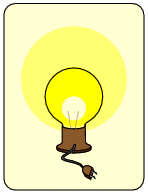
\includegraphics[height=50pt]{Opencircuit.png}
	\end{center}
\end{frame}

\begin{frame}{Companies and institutions}
	\begin{center}
		
\includegraphics[width=100pt]{HKUST_Logo.png}
		
\includegraphics[width=100pt]{NFF.jpg}
		
\includegraphics[width=100pt]{efabless_logo.png}
	\end{center}
\end{frame}

\section[How]{}
\begin{frame}{How we do it}
	\begin{itemize}
		\item Introducing an open source chip manufacturing process standard specification
	\end{itemize}
\end{frame}

\begin{frame}{Help needed}
	\begin{itemize}
		\item Help with QtFlow\footnotemark
		\item Help with the LibreSilicon process\footnotemark
	\end{itemize}
	
	\footnotetext[1]{https://github.com/leviathanch/qtflow}
	\footnotetext[2]{https://github.com/leviathanch/libresiliconprocess}
\end{frame}



\end{document}